% Reset counters and commands for appendix
\setcounter{chapter}{0}
\renewcommand{\thechapter}{\Alph{chapter}}
\setcounter{equation}{0}
\renewcommand{\theequation}{\Alph{chapter}.\arabic{equation}}
\setcounter{figure}{0}
\renewcommand{\thefigure}{\Alph{chapter}.\arabic{figure}}
\setcounter{table}{0}
\renewcommand{\thetable}{\Alph{chapter}.\arabic{table}}
\appendix
\chapter{Macでの研究環境の構築}
ここでは、Macで研究環境を構築する祭に最低限やるべきこと、知っておくべきことを説明します。Macに限らずWindowsやLinuxでも、計算機環境の設定は個々人の好みや研究内容によって大きく変わります。そのため、ここに書くことは参考程度にとどめて下さい。この章での説明は、OS X Lionを前提に書かれており、また使用するスクリーンショットもLion環境のものです。Snow Leopardでは多少異なる可能性があるので注意してください。
\section{英語環境にする}
日本の研究室でMacを使う場合、OSの言語環境を日本語にしている人が多いでしょう。しかしMacを研究で使う場合には英語環境に変更することを強くお勧めします。大きく四つの理由があるからです。

まず第一に、インターネット上のMac関係の情報の多くが英語で書かれており、英語で検索した場合に見つかる情報の量と質は日本語の情報を圧倒するからです。使っているMacで何か問題が生じた場合にエラーメッセージが日本語で表示されていると、それを検索語にしても辿り着ける情報には限りがあります\footnote{\LaTeX 関係などの情報だと日本語特有の問題も発生しうるので、そこは臨機応変に対応して下さい。}。Apple社はアメリカの企業でありMacユーザの多くが北米に集中しています。そのためMac関連の情報のやり取りの多くは英語でなされています。これはMacに限らずコンピュータ関係全般に言えます\footnote{恐らく唯一の例外がRubyというプログラミング言語です。これは日本人により開発されたものが世界に広がった希有な例です。}

第二に、あなたは日本人のみと共同研究をするわけではないからです。もしあなたのMacの画面を外国人が見ながら、もしくはあなたが外国人のMacの画面を見ながら作業する時に、OSが英語環境になっていたほうが意志疎通が簡単になることは言うまでもないでしょう。また海外(特にアメリカ)の研究機関などで実験をするときに、現地で使用するMacが英語環境になっているのは当然です。

第三の理由は、ファイル名やメニューの表示が英語になっているほうが作業効率が上がるからです。Macだとホームディレクトリに「書類」や「デスクトップ」というディレクトリが存在しますが、英語環境ではそれぞれ「Documents」と「Desktop」です。Terminal.appからホームで\texttt{ls}すれば、実体が英語名だということがわかります。Finder.appからディレクトリの移動をしたいときに、英語環境であればホームを開いた状態で「do」と連打すれば「Documents」が選択された状態になります。また「de」と打てば「Desktop」が選択されます。日本語環境の場合だとこうはいきません。またメニューの「編集」は英語環境では「Edit」になっています。メニューで「Edit」を開いた状態で「co」と連打すれば「Copy」のところが選択された状態になるでしょう。

最後の理由は、できる限り英語に慣れ親しんだほうが良いからです。大学院に入りたての頃は、誰しも英語の読み書きと会話に苦労するでしょう。また日本人の多くの研究者はその後何十年も英語で苦労をし続けます。少しでも英語に慣れるため、常用するMacくらい英語環境で使う意志を持ちましょう。

ただし、英語環境にすることで問題が生じる場合があります。例えば英語環境でAdobe Flashを表示すると日本語が文字化けすることがあります。これはFlashが既に廃れつつある技術であり、かつFlashの開発チームが能力不足だからです。他にも英語環境にすると日本語表示がうまくいかないソフトがあるかもしれませんが、そのようなソフトを使うのはやめましょう。日本語表示以外にも色々と問題を抱えている可能性があります。

図\ref{fig_English1_png}から図\ref{fig_English3_png}のように「システム環境設定」から英語環境に変更することができます。この設定後に起動したアプリケーションは、全て英語環境として起動されます。全てのメニューなどが英語で表示されるはずです。図\ref{fig_English3_png}にある「単語区切り」の設定は忘れないようにして下さい。ダブルクリックで日本語文字列を選択する場合に、熟語やカタカナ語が一つの単語として認識されるようになります。

\begin{figure}
  \centering
  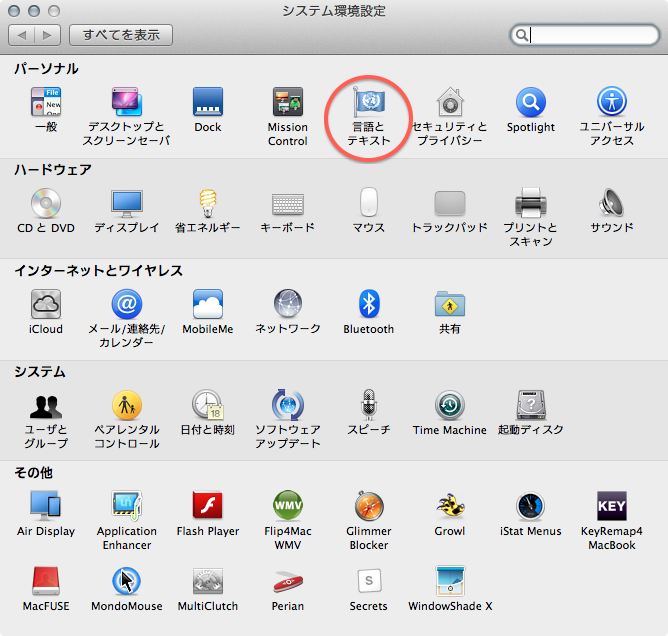
\includegraphics[scale=0.35]{fig/English1.png}
  \caption{「システム環境設定」から「言語とテキスト」を開く}
  \label{fig_English1_png}
\end{figure}

\begin{figure}
  \centering
  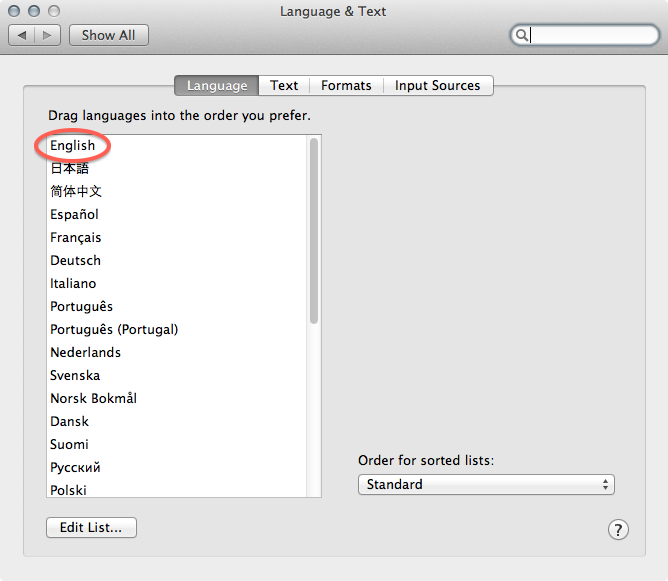
\includegraphics[scale=0.35]{fig/English2.png}
  \caption{「日本語」ではなく「English」を先頭に持ってくる(この画面は既に英語環境になっている場合のもの)}
  \label{fig_English2_png}
\end{figure}

\begin{figure}
  \centering
  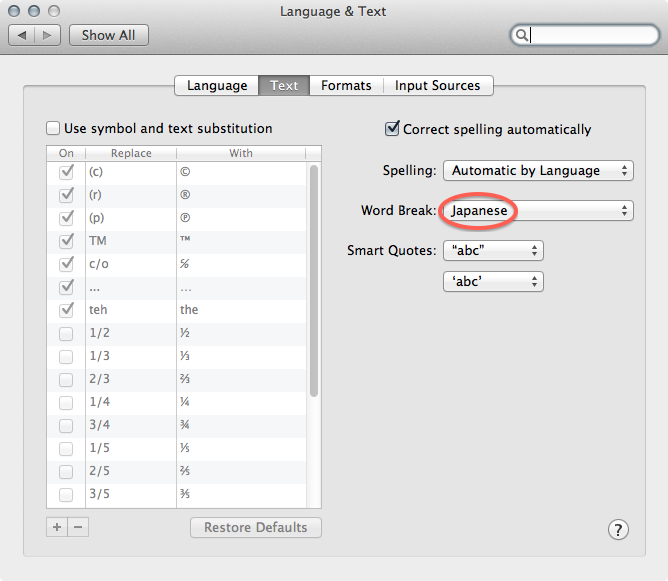
\includegraphics[scale=0.35]{fig/English3.png}
  \caption{「単語区切り(Word Break)」を「Japanese」にする(この画面は既に英語環境になっている場合のもの)}
  \label{fig_English3_png}
\end{figure}


\section{拡張子を表示する}
Macの初期設定では、ファイルの拡張子(extension)が表示されません。図~\ref{fig_Extension_png}のようにFinder.appの「Preferences\ldots」から表示する設定に変更しましょう。この表示をしないと、Terminal.appから操作するファイル名とFinder.appからファイル名が見かけ上一致しない場合があります。

\begin{figure}
  \centering
  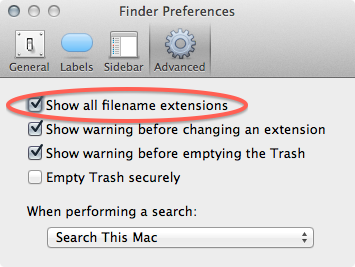
\includegraphics[scale=0.35]{fig/Extension.png}
  \caption{「Show all filename extensions」にチェックを入れると、全てのファイルで拡張子が表示されるようになる}
  \label{fig_Extension_png}
\end{figure}

\section{キーボードの設定}

\subsection{Caps LockキーをControlキーに変更する}
もしあなたのMacがUS配列のキーボードならば、Caps LockキーはControlキーとして機能するように設定を変更しましょう。図\ref{fig_Keyboard1_png}のように、System Preferencesから「Keyboard」を開いて「Keyboard」タブの「Modifier keys\ldots」を押し、Caps LockをControlにします。後述するように、OS~X環境ではEmacsの操作体系に倣ったキーボードショートカットが使われています。そのため、Controlキーの使用率が他のOSに比べて非常に高くなるのが特徴です。US配列のキーボードを使用している場合にはControlキーが押しにくい位置にあるため、滅多に使わない、かつ最も押しやすい位置にあるCaps LockをControlキーにしてしまうことがよく行われています。

\begin{figure}
  \centering
  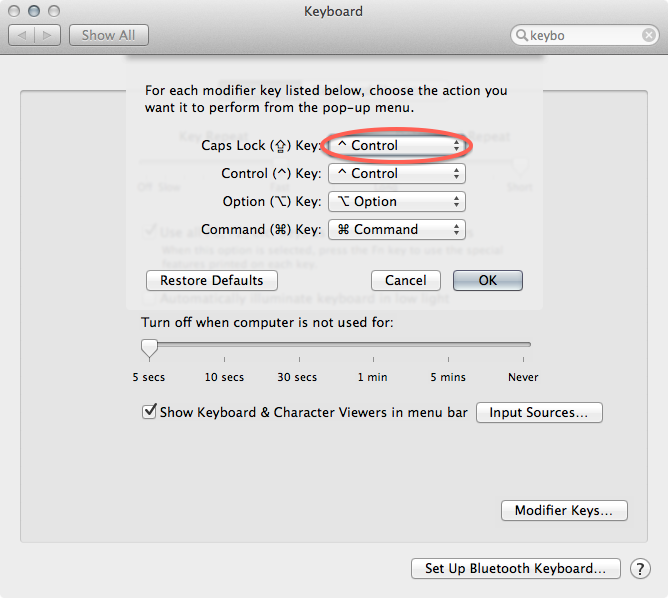
\includegraphics[scale=0.35]{fig/Keyboard1.png}
  \caption{Caps LockをControlキーに変更する}
  \label{fig_Keyboard1_png}
\end{figure}

\subsection{Tabキーの動作の変更}
次に、図\ref{fig_Keyboard2_png}のように「Keyboard Shortcuts」のタブに移動し、ボタンなどの選択を全てTabキーで行えるようにします。このようにすることで、様々な画面操作をするときに、いちいちキーボードからトラックパッドやマウスへ手の移動をしなくて済むようになります。

\begin{figure}
  \centering
  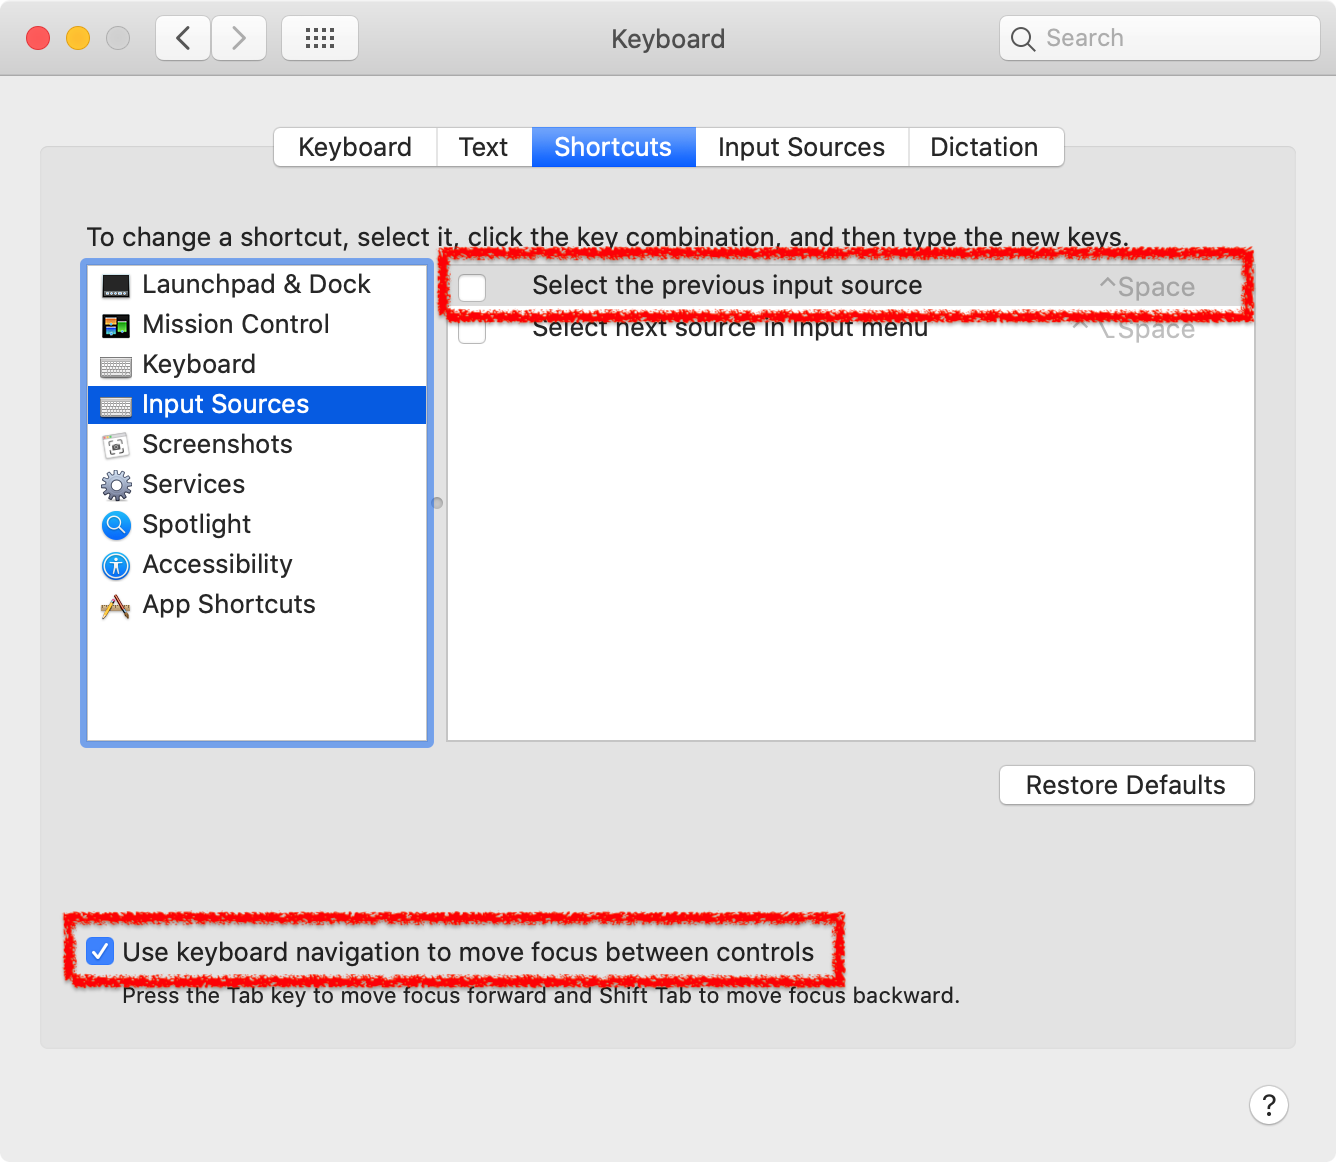
\includegraphics[scale=0.35]{fig/Keyboard2.png}
  \caption{全てのボタンなどをtabキーで移動できるようにする}
  \label{fig_Keyboard2_png}
\end{figure}

例えば、Mac の電源ボタンを軽く一度だけ押すと、図\ref{fig_reboot_png}のような確認ダイアログが出てくるはずです。ここで数回Tabキーを押すと、「Cancel」ボタンが強調表示されるようになります。また「Shut Down」ボタンが明滅しているでしょう。この状態でSpaceキーを押すと、マウスやトラックパッドの操作をしなくても強調表示された「Cancel」ボタンが押されます。またReturnキーを押すと明滅している「Shut Down」ボタンが押されてMacが再起動します。このように、Macではダイアログのボタンをクリックする代わりにSpaceキーとReturnキーで操作することができます。

\begin{figure}
  \centering
  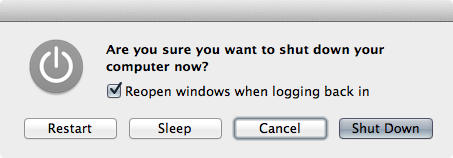
\includegraphics[scale=0.35]{fig/reboot.png}
  \caption{再起動の確認ダイアログ。Tabを数回押すと、「Cancel」が強調表示される。「Shut Down」は明滅している。}
  \label{fig_reboot_png}
\end{figure}

\subsection{Spotlightのショートカットの変更}
最後に、Spotlightのショートカットを図\ref{fig_Keyboard3_png}のようにControl-Space(画面上の表示は「\verb|^|Space」)の組み合わせからCommand-Space(画面上の表示は「\cmd{}Space」)などの組み合わせに変更しましょう。Control-Spaceは後述するようにEmacsで頻繁に使用するショートカットであるため、Spotlightのショートカットとして使用されてしまうと不便だからです。

Command-SpaceをSpotlightにあてがってしまうと、文字入力の日本語と英語の切り替えはどうするのかと、Macに少し慣れた人なら疑問に思うかもしれません。しかし最近のMacにはJIS配列の場合「かな」と「英数」キーが存在するため、これらのキーを使ったほうが文字入力の切り替えは簡単に行えます。またUS配列のMacを使っている場合には、\ref{sec_KeyRemap4MacBook}にて後述するKeyRemap4MacBookを使うことで「かな」と「英数」をCommandキーに割り当てることが可能になるため、やはりCommand-Spaceのショートカットは不要です。

\begin{figure}
  \centering
  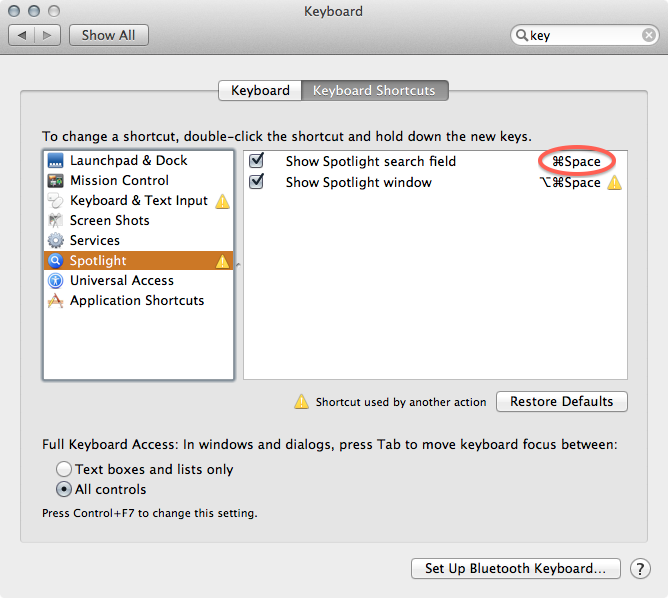
\includegraphics[scale=0.35]{fig/Keyboard3.png}
  \caption{Spotlightのショートカットを「Control-Space」から「Command-Space」に変更した状態}
  \label{fig_Keyboard3_png}
\end{figure}

\section{KeyRemap4MacBook}
\label{sec_KeyRemap4MacBook}

\ref{sec_Emacs}で述べるように、OS Xのキーボード操作の多くはEmacsの操作体系に基づいています。しかし、この操作に対応していないアプリケーションも存在するため(Microsoft製品、Adobe製品、Eclipseなど)、KeyRemap4MacBook\footnote{\url{http://pqrs.org/macosx/keyremap4macbook/index.html.ja}}をインストールすることでOS Xの操作を快適にすることができます。

KeyRemap4MacBookをインストール後、「System Preferences」から「KeyRemap4MacBook」の「Change Key」タブを開くと、図\ref{fig_KeyRemap4MacBook1_png}のような画面が現われます。大量の設定項目が存在しますが、そのうち、「Control+D to Forward Delete」、「Control+H to Delete」、「Control-I to Tab」、「Control+M to Return」、「Control+PNBF to Up/Down/Left/Right」、「Control+V to PageDown」などを動作させると良いでしょう。

\begin{figure}
  \centering
  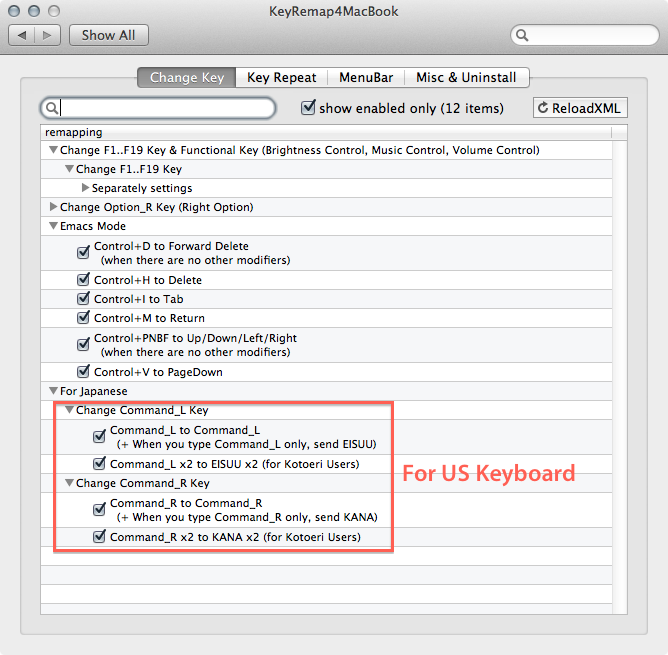
\includegraphics[scale=0.35]{fig/KeyRemap4MacBook1.png}
  \caption{OS Xのほとんどの操作で、Emacsに似た操作体系を実現するための設定の例。USキーボードの使用者は、赤枠内の設定も追加することで日本語入力が楽になる。}
  \label{fig_KeyRemap4MacBook1_png}
\end{figure}

また、JIS配列のキーボードではなく、US配列のものを使用している人の場合、「Command\_L to Command\_L」、「Command\_L x2 to EISUU x2」、「Command\_R to Command\_R」、「Command\_R x2 to KANA x2」を動作させておけば、左右のCommandキーを英数キー、かなキーとして使用することが可能になります。もちろん、他のキーと組み合わせた場合にはCommandキーとしても動作します。

次に、「Key Repeat」タブを開くと「[Key Repeat] Wait」という設定項目があります。ここの時間を短くすることで、キーを押下し続けたときに繰り返し入力される時間間隔を短くすることが可能です。あなたがMacやEmacsの操作に熟達する頃には、デフォルトの$80$ミリ秒では遅過ぎると感じるようになっているはずです。

\begin{figure}
  \centering
  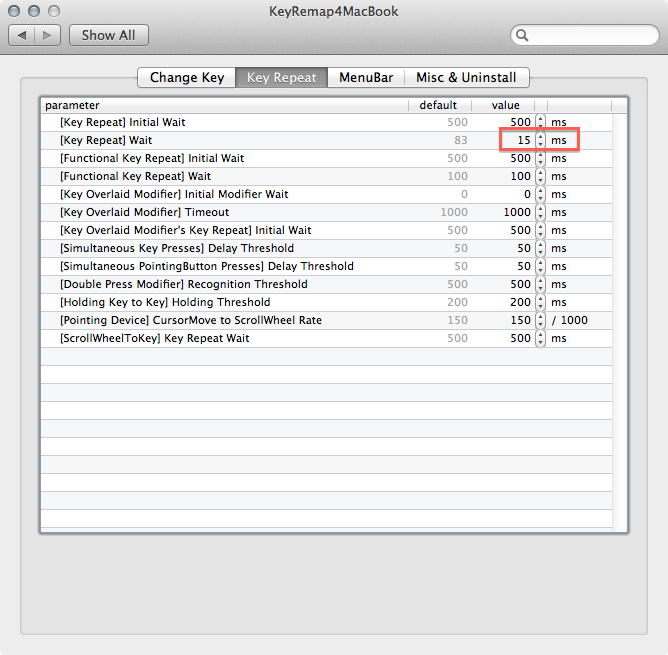
\includegraphics[scale=0.35]{fig/KeyRemap4MacBook2.png}
  \caption{キーボードを押下し続けた場合の繰り返し入力の設定}
  \label{fig_KeyRemap4MacBook2_png}
\end{figure}

\section{zsh}

OS Xの標準のshell環境は、Snow LeopardやLionではbashになっています。bashはLinuxやOS Xで広く使われており、ソフトウェアの一部やOSの設定スクリプトなどで見ることができます。cshやtcshを使う人も少なくない数が存在しますが、2012年現在でMacを研究に使うにはbashを選択するのが標準的です。

一方で、bashよりも更に高機能なshellとして最近ではzshの人気が高まっています。zshはbashの文法に非常に似ているものの、独自の拡張機能をたくさん持っているため、bashに慣れている人には「便利なbash」として使うことが可能です。また、初学者の場合はbashとzshの違いは全く気にする必要はないでしょうから、bashではなくzshを使い始めるのが良いでしょう。

図\ref{fig_zsh1_png}と図\ref{fig_zsh2_png}に、shellをzshに変更する方法を説明します。まず図\ref{fig_zsh1_png}のように、「System Preferences」の「Users \& Groups」を表示し、自分のアカウントを右クリック(トラックパッドの場合は二本指クリック)します。「Advanced Options\ldots」が現われるので、これを選択します。ウィンドウ左下の鍵マークがロックされている状態の場合は右クリックが効きませんので、パスワードを入力してこれを解除して下さい。

\begin{figure}
  \centering
  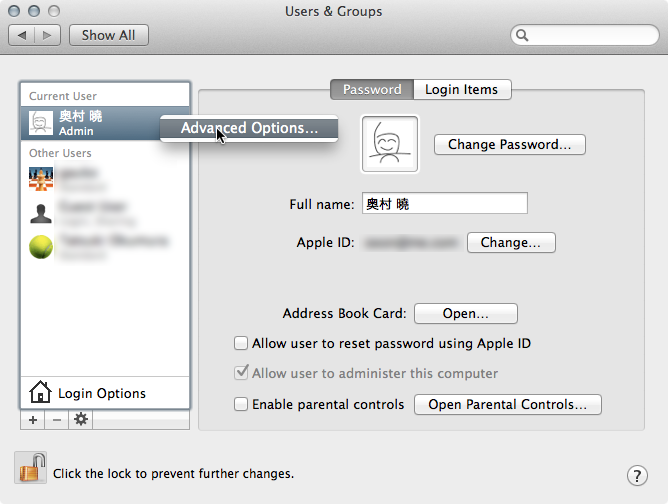
\includegraphics[scale=0.35]{fig/zsh1.png}
  \caption{自分のアカウントを右クリックして「Advanced Options\ldots」を表示する}
  \label{fig_zsh1_png}
\end{figure}

図\ref{fig_zsh2_png}が表示されるので、「Login shell」を「/bin/bash」から「/bin/zsh」に書き換えて下さい。ここで、{\bf{\textgt{絶対に打ち間違えをしないように注意してください}}}。これで、次にTerminalを開くときから、ログインshellがzshに変更されます。

\begin{figure}
  \centering
  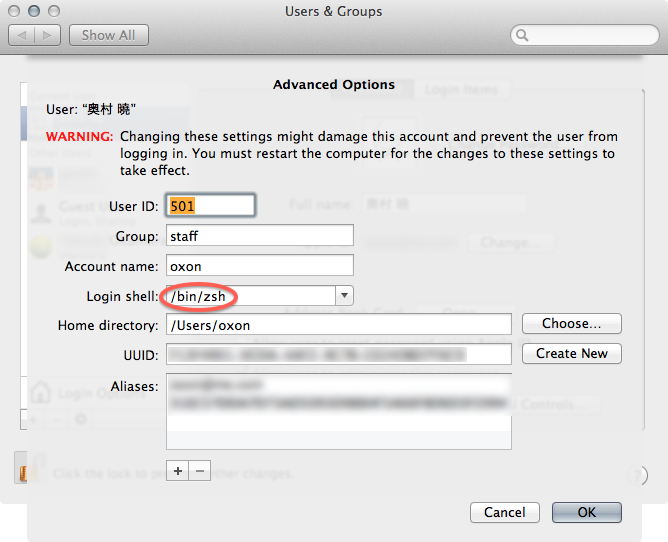
\includegraphics[scale=0.35]{fig/zsh2.png}
  \caption{「/bin/bash」を「/bin/zsh」に書き換える}
  \label{fig_zsh2_png}
\end{figure}

bashからzshに変更すると、各種の設定は\texttt{\$HOME/.bashrc}ではなく\texttt{\$HOME/.zshrc}に書くようになります。例えば次の設定を\texttt{\$HOME/.bashrc}に書けと指示があった場合、\texttt{\$HOME/.zshrc}にこれを書いて下さい。

\begin{lstlisting}[language=bash]
export ROOTSYS=/usr/local/root
\end{lstlisting}

zshの設定や\texttt{\$HOME/.zshrc}の書きかたについては、「漢のzsh\footnote{\url{http://news.mynavi.jp/column/zsh/index.html}}」というコラムの解説が非常に詳しく分かりやすいので、参考にして下さい。

\section{MacPorts}
\label{sec_MacPorts}
MacPorts\footnote{\url{http://www.macports.org/}}とは、UNIXやLinuxで広く使われ、また開発の行われてきたソフトウェア資産を、Macでも使えるようにするためのプロジェクトのひとつです。GUIソフトウェアでもそうですが、他の環境で動作するソフトウェアだからと言って、Macでも簡単に動くわけではありません。Mac以外のUNIXに書かれたソフトウェアであっても、Mac用にコンパイルしたり、各種設定を変更してやる必要があります。しかしMacPortsのようにMacに移植するプロジェクトの成果を利用することで、難しい作業を一般ユーザが行う必要がなくなります。

同様のプロジェクトに、Fink\footnote{\url{http://www.finkproject.org/}}やHomebrew\footnote{\url{http://mxcl.github.com/homebrew/}}があります。OS Xのリリース初期ではFinkが最も活発でしたが、ROOTと組み合わせた場合に問題が何度か発生したため、筆者はMacPortsに移行しました。最近ではHomebrewが流行っていますが、MacPortsに比べるとまだユーザ数は多くありません。新しもの好きの人はHomebrewを検討してみて下さい。

\subsection{MacPortsの導入}

MacPortsをダウンロードし、Macの他のソフトウェアと同様にインストーラを使ってインストールします。MacPorts本体と、関連するコマンド、ライブラリ、ヘッダーファイルなどは全て\texttt{/opt}にインストールされます。以下の設定を\texttt{\$HOME/.zshrc}に追加して下さい。
\begin{lstlisting}[language=bash]
export PATH=/opt/local/bin:$PATH
export LD_LIBRARY_PATH=/opt/local/lib:$LD_LIBRARY_PATH
export C_INCLUDE_PATH=/opt/local/inc:$C_INCLUDE_PATH
export CPLUS_INCLUDE_PATH=/opt/local/inc:$C_INCLUDE_PATH
\end{lstlisting}

Terminalから、次のコマンドを実行して\texttt{\$HOME/.zshrc}の設定を反映しましょう。新しいTerminalを開いた場合は、いちいち実行する必要はありません。

\begin{lstlisting}[language=bash]
$ source ~/.zshrc
\end{lstlisting}

MacPortsで好きなソフトウェアをインストールするには、いくつかコマンドを実行する必要があります。Emacsの導入事例を\ref{sec_Emacs}で説明します。

\subsection{Emacs}

まず、MacPortsでEmacsをインストールできるかどうか調べてみましょう。次のコマンドで説明文中に「emacs」の含まれるソフトウェア(port)があるか確認します。

\begin{lstlisting}[language=bash]
$ port search emacs
\end{lstlisting}

そうすると、たくさんの出力が次のように表示されるはずです。これを細かく見ていくと、「GNU Emacs」という文字列を含んだportがいくつか存在するはずです。

\begin{lstlisting}
auctex @11.86 (editors, print)
    A major emacs mode for editing TeX files.
(snip)
emacs @23.4 (editors)
    The GNU Emacs text editor

emacs-app @23.4 (aqua, editors)
    The GNU Emacs text editor (Cocoa version)

emacs-app-devel @20091101 (aqua, editors)
    The GNU Emacs text editor, recent CVS development version

emacs-snapshot @20120423 (editors)
    The GNU Emacs text editor

emacs-w3m @1.4.4 (www)
    Use the w3m web browser inside emacs.

emacs22 @22.3 (editors)
    The GNU Emacs text editor
(snip)
zile @2.3.23 (editors)
    Zile Is Lossy Emacs

Found 38 ports.
\end{lstlisting}

「emacs @23.4 (editors)」というのが、バージョン23.4のEmacsだと検討がつくので、さらに次のコマンドで詳細を見てみましょう。

\begin{lstlisting}[language=bash]
$ port info emacs
\end{lstlisting}

次のように、説明が何行も表示されます。
\begin{lstlisting}
emacs @23.4, Revision 1 (editors)
Variants:             dbus, gtk, motif, universal, x11

Description:          GNU Emacs is a self-documenting, customizable, extensible
                      real-time display editor. Users new to Emacs will be able
                      to use basic features fairly rapidly by studying the
                      tutorial and using the self-documentation features. Emacs
                      also has an extensive interactive manual browser. It is
                      easily extensible since its editing commands are written
                      in Lisp.
Homepage:             http://www.gnu.org/software/emacs/emacs.html

Build Dependencies:   pkgconfig, texinfo
Library Dependencies: ncurses
Conflicts with:       xemacs
Platforms:            darwin, freebsd
License:              GPL-3+
Maintainers:          dports@macports.org, openmaintainer@macports.org
\end{lstlisting}

実は、OS Xには最初からEmacsがインストールしてあるため、必ずしもEmacsを自分でインストールする必要はありません。しかし、OS Xに含まれるEmacsはX11に対応していないため、Terminalの中でしかEmacsを立ち上げることはできません。一方、MacPortsの場合にはX11に対応したEmacsをインストールすることが可能です。研究をする上では、こちらのほうが便利なのでMacPortsでEmacsを導入しましょう。

ここで、「Variants:」と書かれた説明を見ると、「x11」とあるのが分かります。EmacsをMacPortsでインストールするときに、どのようなオプションが選択可能かを示しており、この場合は「x11」というオプションを指定すればX11に対応したEmacsがインストールされることを示しています。

次のコマンドを実行し、X11に対応したEmacsをインストールしましょう。管理者パスワードを要求されます。

\begin{lstlisting}[language=bash]
$ sudo port install emacs +x11
\end{lstlisting}

インストールが開始されると、Emacsを使うために必要な他のportもインストールされます。以下のような出力が表示されれば、Emacsを使えるようになっているはずです。

\begin{lstlisting}
--->  Fetching archive for zlib
--->  Attempting to fetch zlib-1.2.7_0.darwin_11.x86_64.tbz2 from http://packages.macports.org/zlib
--->  Attempting to fetch zlib-1.2.7_0.darwin_11.x86_64.tbz2.rmd160 from http://packages.macports.org/zlib
--->  Installing zlib @1.2.7_0
--->  Cleaning zlib
(snip)
--->  Computing dependencies for emacs
--->  Fetching archive for emacs
--->  Attempting to fetch emacs-23.4_1.darwin_11.x86_64.tbz2 from http://packages.macports.org/emacs
--->  Attempting to fetch emacs-23.4_1.darwin_11.x86_64.tbz2.rmd160 from http://packages.macports.org/emacs
--->  Installing emacs @23.4_1
--->  Activating emacs @23.4_1

D-Bus support is no longer included in the default Emacs installation. To build
Emacs with D-Bus support, please install with the +dbus variant.

--->  Cleaning emacs
\end{lstlisting}

LionでXcode 4.3を使っている場合に次のようなエラーが表示されるかもしれません。

\begin{lstlisting}
Error: 
Error: No valid Xcode installation is properly selected.
Error: Please use xcode-select to select an Xcode installation:
Error:     sudo xcode-select -switch /Applications/Xcode.app/Contents/Developer # version 4.3.2
Error: 
Warning: xcodebuild exists but failed to execute
Warning: Xcode does not appear to be installed; most ports will likely fail to build.
\end{lstlisting}

そのときは、エラーの指示通りに従い、次のコマンドを実行しましょう。これでMacPortsが動作するようになるはずです。
\begin{lstlisting}[language=bash]
$ sudo xcode-select -switch /Applications/Xcode.app/Contents/Developer
\end{lstlisting}

\subsection{\LaTeX}

研究で誰しも必要になるのが\LaTeX{}の環境です。様々なインストール方法があり、インターネット上にも色々な情報が散らばっています。MacPortsから\LaTeX{}を入れる場合でも、ptex、tetex、texliveという三つのportが存在します。

\begin{lstlisting}
$ port info ptex   
pTeX @20110314, Revision 1 (tex, print, textproc, japanese)
Variants:             euc, [+]motif, nextaw, no_hiragino, no_otf, no_x11, sjis,
                      [+]utf8, xaw, xaw3d

Description:          Japanese TeX (pTeX) processing environment
Homepage:             http://www.nn.iij4u.or.jp/~tutimura/tex/ptetex.html

Build Dependencies:   ghostscript-fonts-hiragino, nkf
Library Dependencies: gd2, jpeg, libiconv, libpaper, libpng, ncurses, perl5,
                      t1lib, zlib, openmotif
Runtime Dependencies: ghostscript-fonts-hiragino, t1utils, texi2html, texinfo
Conflicts with:       texlive-common
Platforms:            darwin
License:              Restrictive/Distributable
Maintainers:          takanori@macports.org, openmaintainer@macports.org
\end{lstlisting}

Macで\LaTeX{}を使う場合、文字コードをUTF-8にするのが標準的です。ptexでは特に指定しない限りはUTF-8に対応したものがインストールされるため、「Variants:」の説明に「[+]utf8」と書いてあります。

次のコマンドでptexを入れましょう。\texttt{platex}、\texttt{pdflatex}、\texttt{dvipdfmx}などのコマンドが一緒にインストールされます。好みに応じて、代わりにtexliveやtetexを導入するのでも良いでしょう\footnote{違いが何なのかは筆者は理解していません。}。

\begin{lstlisting}[language=bash]
$ sudo port install ptex
\end{lstlisting}

\section{Emacsの操作体系に慣れる}
\label{sec_Emacs}

ここでは、OS Xでの標準的なエディタ(editor)のひとつであるEmacsの操作について、その初歩の初歩について説明します。エディタは文章を書くためのソフトウェアです。ただし、ワープロのように様々な装飾をするための機能はありません。プログラムを書いたり、\LaTeX{}のソースを書いたりと、装飾ではなく文そのものに意味があるときに使います。そのような作業に特化したワープロにはない様々な機能が搭載されています。

Emacsの特徴のひとつに、文字入力に特殊なキーボードショートカット(Emacs key binding)を使うことが挙げられます。慣れないうちは全く便利に感じないと思いますが、一度慣れてしまうと、もう他のエディタには戻れなくなるのでぜひ覚えて下さい。OS Xを使う場合、このショートカットをほとんどのソフトウェアでも利用可能です。例えば、OS Xに標準で付属しているメールクライアント「Mail」でメッセージを編集する時にも、このショートカットが使用できます。基本的なキーボードショートカットの一覧を表\ref{tab_emacs}にまとめました。

\begin{table}
  \centering
  \caption{Emacsの基本的なキーボードショートカット}
  \label{tab_emacs}
  \begin{tabular}{llp{10cm}}
  \hline
ショートカット & 英単語 & 機能 \\ \hline\hline
C-f & {\bf F}orward & 一文字進む(→キーと同等) \\
C-b & {\bf B}ackward & 一文字戻る(←キーと同等) \\
C-p & {\bf P}revious line & 次の行へ進む(↓キーと同等) \\
C-n & {\bf N}ext line & 前の行へ戻る(↑キーと同等) \\
C-a & {\bf A}head & 行頭へ移動 \\
C-e & {\bf E}nd & 行末へ移動 \\
C-k & {\bf K}ill & カーソル位置から行末までを全て kill-ring と呼ばれるメモリ領域に移動(カットに類似) \\
C-y & {\bf Y}ank & kill-ringにあるものをカーソル位置にペースト \\
C-t & {\bf T}ranspose & カーソルの前後の文字を入れ替える \\
C-h & 不明 & カーソル前方を一文字削除(MacのDelete、WindowsのBackspaceと同等) \\
C-d & forward {\bf D}elete & カーソル後方を一文字削除(WindowsのDeleteと同等) \\
C-m & 不明 & 改行(カーソルも次の行へ移動する) \\
C-o & 不明 & 改行(カーソルは元の位置にとどまる) \\
C-Space C-w & 不明 & C-Space入力時のカーソル位置から、C-w入力時のカーソル位置までの範囲をkill-ringに移動する \\ \hline
C-x C-f & {\bf F}ind file & 既存ファイルを開く、なければ作成する \\
C-x C-s & {\bf S}ave & ファイルを保存する \\
C-x C-c & 不明 & 終了する \\
C-x C-w & 不明 & ファイルを別名で保存する \\
C-x C-2 & 不明 & ウインドウを二分割にする \\
C-x C-1 & 不明 & ウインドウを一分割にする \\
C-s & {\bf S}earch & 検索する \\
C-r & {\bf R}verse search & 後方に検索する \\
M gg & 不明 & 特定の行に移動する\\\hline
  \end{tabular}
\end{table}

まずはEmacsを次のコマンドで起動してみましょう。MacPortsからEmacsを入れていなかったり、MacPortsで「+x11」をつけずにEmacsをインストールした場合には図\ref{fig_emacs_nox11_png}のような表示が現われるはずです\footnote{X11に対応したEmacsでも、「-nw」という引数をつけてEmacsを起動すれば、同様の表示にすることが可能です。接続速度の遅い(つまり画像を飛ばすのが遅い)SSHの接続先などで作業する場合に使うこともあります。}。

\begin{lstlisting}[language=bash]
$ emacs
\end{lstlisting}

\begin{figure}
  \centering
  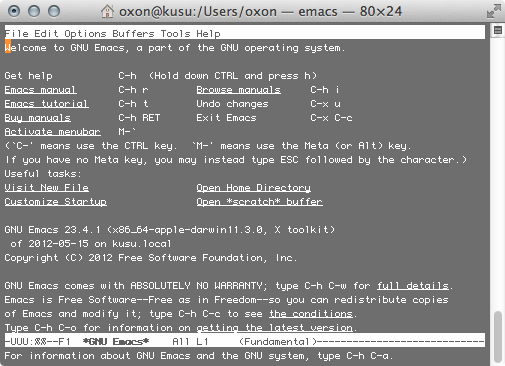
\includegraphics[scale=0.35]{fig/emacs_nox11.png}
  \caption{X11対応でないEmacsの起動例}
  \label{fig_emacs_nox11_png}
\end{figure}

X11に対応したEmacsを起動した場合は、図\ref{fig_emacs1_png}のようなウィンドウが表示されます。まずは、新しいファイルを作成してみましょう。Controlキーを左手小指で押下し、左手中指でXキーを同時に押します。その後、Controlキーを押した状態のまま左手人さし指でFキーを同時に押します。これを、「C-x C-f」のように表記します\footnote{Control-x、Ctl-x、Cn-xなど、いくつかの表記方法があります。好みの問題です。}。表\ref{tab_emacs}にあるように、これは新規ファイルを作成するためのショートカットです。図\ref{fig_emacs2_png}のように「Find file:」の後に続けて作成したいファイル名を入力しましょう。図\ref{fig_emacs2_png}では\texttt{~/foo.txt}を作成しています。

\begin{figure}
  \centering
  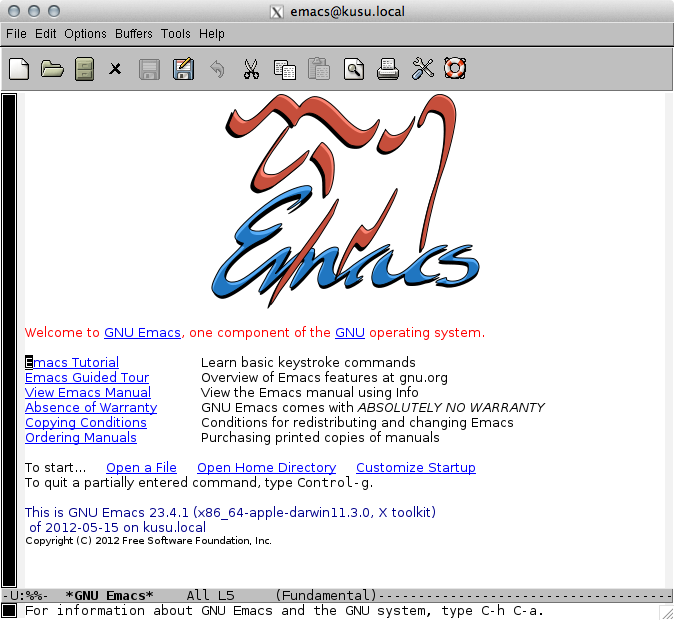
\includegraphics[scale=0.35]{fig/emacs1.png}
  \caption{X11対応のEmacsの起動例}
  \label{fig_emacs1_png}
\end{figure}

\begin{figure}
  \centering
  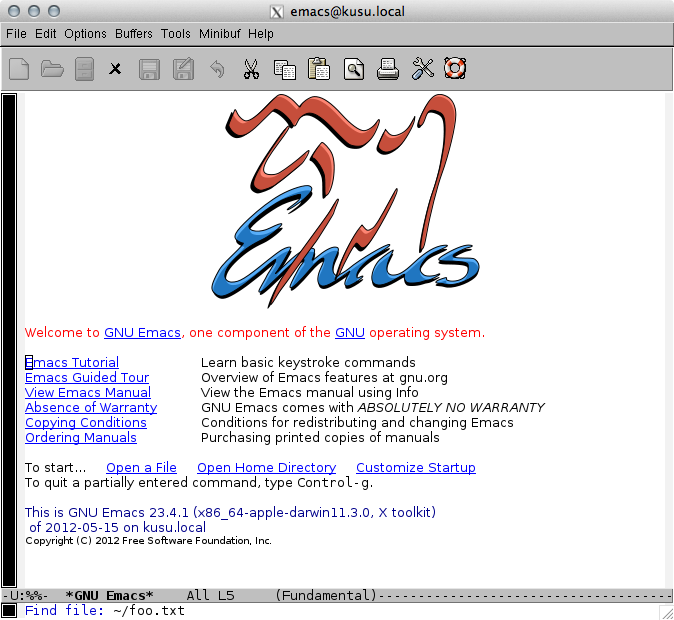
\includegraphics[scale=0.35]{fig/emacs2.png}
  \caption{Emacsで新規ファイルを作成する}
  \label{fig_emacs2_png}
\end{figure}

あらたなファイルが作成されたので(保存はされていません)、図\ref{fig_emacs3_png}のように文字を入力しましょう。この後、C-x C-s を入力すると実際にディスク上に保存されます。図\ref{fig_emacs3_png}の下部に「Wrote /Users/oxon/foo.txt」と表示されます。最後に、C-x C-cと入力してEmacsを終了しましょう。

\begin{figure}
  \centering
  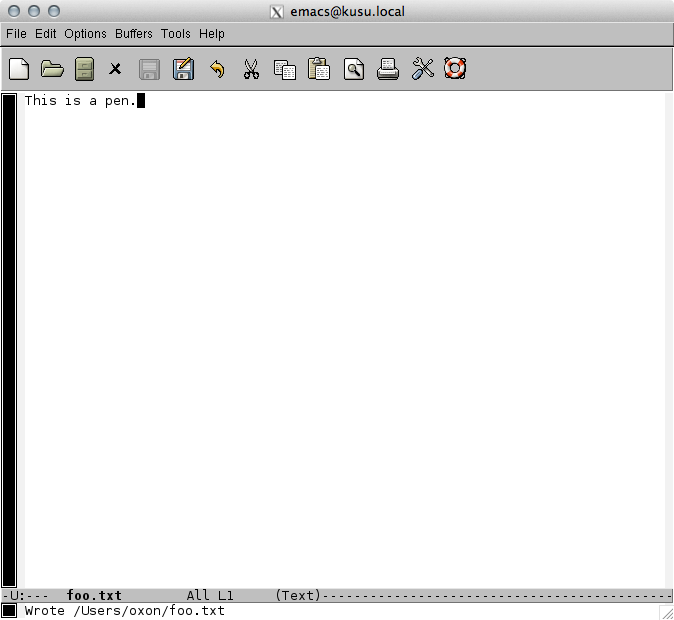
\includegraphics[scale=0.35]{fig/emacs3.png}
  \caption{Emacsで文字入力をし、保存する}
  \label{fig_emacs3_png}
\end{figure}

Emacsの操作に慣れるには、まずこのControlキーを多用した操作に慣れることが重要です。表\ref{tab_emacs}に挙げたショートカットを中心にまずは覚え、どのような操作や機能、設定があるのかを調べていきましょう。多機能過ぎて、うんざりするはずです。

\section{C-Space C-wをOS Xで使う}

表\ref{tab_emacs}に示したショートカットの多くはOS Xのアプリケーションでも使うことができます。また使えないアプリケーションでも、\ref{sec_KeyRemap4MacBook}に書いたようにKeyRemap4MacBookの設定で使用可能になります。

しかし、デフォルトの状態ではC-Space C-wはOS Xのアプリケーションでは使うことができません。Emacsに慣れてくると、C-Space C-wがEmacs以外で使えないのが不便に感じるでしょう。OS Xにはこの操作を実現するための機能が隠されています。

コード\ref{code_DefaultKeyBinding}を、\texttt{\~{}/Library/KeyBindings/DefaultKeyBinding.dict}として保存して下さい\footnote{\url{http://akenox.dip.jp/index.php?Translations\%2FMac\%20OS\%20X\%20Key\%20Bindings}に詳しい解説がある。}。「Mail」などを起動して文字入力する際に、C-Space C-wやC-x C-sが有効になっているはずです\footnote{Lionからは「Save As\ldots」が「Duplicate」などに置き換わってしまったため、コード\ref{code_DefaultKeyBinding}の設定をしてもC-x C-wは動作しません。}。

%\begin{NoFloat}
\lstinputlisting[float=tb,caption=\texttt{DefaultKeyBinding.dict},label=code_DefaultKeyBinding,numbers=left]{src/DefaultKeyBinding.dict}
%\end{NoFloat}

\section{Xcode}

\section{知っていると便利な OS X 特有のコマンド}

\chapter{configure と Make}

OS XやLinux環境でソフトウェアを導入する時、インストールの方法は主に3つあります。1つ目は、\ref{sec_MacPorts}で説明したようなパッケージ管理ソフト\footnote{OS XではMacPorts、Fink、Homebrewなど、LinuxではYumやAPTなど。}を使う方法す。2つ目は、既にコンパイル済みでバイナリ配布されているソフトを導入する方法です。例えば、KeyRemap4MacBookをインストーラを使ってインストールしたのがこれに当たります。また、ROOTを入れる場合でもバイナリ配布されているものを使うことが可能です。3つ目は、ソースコードの配布されているソフトウェアを自分でコンパイル(compile)する\footnote{ビルド(build)するとも言います。}方法です。これは\ref{sec_ROOT_install}でROOTの導入として説明しました。

自分でソフトウェアをソースコードからコンパイルする場合、標準的なやり方が存在します。また、研究で通常使うソフトウェアの多くがこの標準的な方法に則して作成されています。そのためここで説明する方法を覚えておけば、多くのソフトウェアを自分で簡単にインストールできるようになります。

このやり方を覚えるために、「GNU Hello\footnote{\url{http://www.gnu.org/software/hello/}}」と呼ばれるソフトウェアを試しにインストールしてみましょう。この「GNU Hello」は標準的な方法を学ぶ上で最適なもので、インストールしても実用性はありません。

まず、次のコマンドで\url{http://ftp.gnu.org/gnu/hello/}から最新版の\texttt{hello-2.8.tar.gz}を落としてきて展開します。展開されたディレクトリに移動して\texttt{ls}で中身を見てみましょう。

\begin{lstlisting}[language=bash]
$ curl -O http://ftp.gnu.org/gnu/hello/hello-2.8.tar.gz
  % Total    % Received % Xferd  Average Speed   Time    Time     Time  Current
                                 Dload  Upload   Total   Spent    Left  Speed
100  681k  100  681k    0     0   150k      0  0:00:04  0:00:04 --:--:--  166k
$ tar zxf hello-2.8.tar.gz
$ cd hello-2.8 
$ ls
ABOUT-NLS      INSTALL        THANKS         configure.ac   man
AUTHORS        Makefile.am    TODO           contrib        po
COPYING        Makefile.in    aclocal.m4     doc            src
ChangeLog      NEWS           build-aux      lib            tests
ChangeLog.O    README         config.in      m4
GNUmakefile    README-release configure      maint.mk
\end{lstlisting}

ここで重要なのは、\texttt{README}、\texttt{INSTALL}、\texttt{configure}の3つです。\texttt{README}は、そのソフトウェアに関する全般的な説明が書かれています。\texttt{INSTALL}には、そのソフトウェアのインストール方法が書かれています。\texttt{less}コマンドなどで、試しに中身を読んでみて下さい。

\begin{lstlisting}[language=bash]
$ less README
$ less INSTALL
\end{lstlisting}

\texttt{configure}はシェルスクリプトで、そのソフトウェアをコンパイルするときに必要なライブラリやコマンドが存在するかどうか、存在するパスはどこか、OSの環境は何かを自動的に調べて必要な設定をしてくれます。また、必要に応じてユーザが様々なオプションを指定することができます。どのようなオプションがあるかは、次のようにヘルプを表示することで読むことができます。

\begin{lstlisting}[language=bash]
$ ./configure --help
\end{lstlisting}

様々なオプションが表示されますが、このうち最も頻繁に使われるのがインストール先の指定のオプション\texttt{--prefix}です。次のように\texttt{configure}を実行することで、\texttt{hello}コマンドを\texttt{/usr/local/bin}にインストールし、またマニュアルを\texttt{/usr/local/share/man/man1}にインストールします。もし\texttt{/usr/local}の代わりに他の場所をしていすれば、これらのファイルは指定した場所の下にインストールされます。
\begin{lstlisting}[language=bash]
$ ./configure --prefix=/usr/local
\end{lstlisting} 

\texttt{configure}が問題なく実行されれば、\texttt{Makefile}というファイルが新たに生成されているはずです。このファイルの中には、そのソフトウェアをどのような手順でコンパイルすれば良いかが全て書かれています。ユーザはどのようなソースコードがあるのかなどを気にする必要はありません。この\texttt{Makefile}の手順の通りに自動的にソフトウェアをコンパイルするには、以下の
コマンドを打つだけです。

\begin{lstlisting}[language=bash]
$ make -j 4
\end{lstlisting} 

\texttt{make}コマンドが\texttt{Makefile}の中身を自動的に調べ、そこに書かれている手順を追ってコンパイルを行います。\texttt{-j 4}のオプションは、使っているCPU能力を最大限に引き出すためのものです。この場合、4コアのCPUを全て使ってくれます。

これで必要なファイルが全て生成されたので、最後にインストール作業を行います。通常は\texttt{/usr/local}にインストールする場合に管理者権限が必要なので、次のコマンドを実行します。

\begin{lstlisting}[language=bash]
$ sudo make install
Password:
\end{lstlisting}

これで、\texttt{/usr/local/bin/hello}などが配置されたはずです。では、確認のため\texttt{hello}を実行しましょう。 
\begin{lstlisting}[language=bash]
$ hello
Hello, world!
\end{lstlisting}

どのようなオプションを渡せるかは、\texttt{--help}や\texttt{-h}をつけて確認します。
\begin{lstlisting}[language=bash]
$ hello -h
Usage: hello [OPTION]...
Print a friendly, customizable greeting.

  -h, --help          display this help and exit
  -v, --version       display version information and exit

  -t, --traditional       use traditional greeting format
  -n, --next-generation   use next-generation greeting format
  -g, --greeting=TEXT     use TEXT as the greeting message

Report bugs to: bug-hello@gnu.org
GNU Hello home page: <http://www.gnu.org/software/hello/>
General help using GNU software: <http://www.gnu.org/gethelp/>
\end{lstlisting}

また\texttt{hello}コマンドのマニュアルを見るには\texttt{man}コマンドを使います。

\begin{lstlisting}[language=bash]
$ man hello
\end{lstlisting}

\chapter{パッケージ管理ソフトウェア}
\ref{chap_package}
\section{\texttt{yum}}
\section{\texttt{homebrew}}


\chapter{本文で登場したROOTスクリプトのPyROOT版}
ここでは、本文中で登場したROOTスクリプトをPyROOTで書き換えた例を掲載します。\texttt{foo.C}というROOTスクリプトであれば、\texttt{foo.py}というPyROOTスクリプトにしてあります。

\begin{NoFloat}
\lstinputlisting[language=python,breaklines=true,caption=\texttt{population.py},label=code_population_py,numbers=left]{src/population.py}
\end{NoFloat}
